\def\year{2017}\relax

\documentclass[letterpaper]{article}
\usepackage{aaai17}
\usepackage{times}
\usepackage{helvet}
\usepackage{courier}
\usepackage{amsmath}
\usepackage{amsfonts}
\usepackage{multirow}
\usepackage{graphicx}
\graphicspath{ {images/} }
\frenchspacing
\setlength{\pdfpagewidth}{8.5in}
\setlength{\pdfpageheight}{11in}
\pdfinfo{
/Title (Bayesian Optimisation of Machine Learning Algorithms)
/Author ()}
\setcounter{secnumdepth}{1}
\DeclareMathOperator*{\argmax}{arg\,max}
 \begin{document}
% The file aaai.sty is the style file for AAAI Press
% proceedings, working notes, and technical reports.
%
\title{Bayesian Optimisation of Machine Learning Algorithms}
\author{
National University of Singapore \\
CS4246 Group 7 \AND
\normalsize\normalfont\textbf{Cheong, Xuan Hao Filbert A0121261Y} \\
\normalsize\normalfont\textbf{Gay, Ming Jian Davis A0111035A} \\
\normalsize\normalfont\textbf{Karen Ang Mei Yi A0116603R} \And
\normalsize\normalfont\textbf{Quek, Chang Rong Sebastian A0121520A} \\
\normalsize\normalfont\textbf{Vincent Seng Boon Chin A0121501E} \\
\normalsize\normalfont\textbf{Xu, Ruofan A0100965J}
}

\maketitle
\begin{abstract}
Machine learning algorithms have grown in popularity over the past few years.
This increased interest and usage also implies an increasing need for
hyperparameter tuning. Traditionally done by human experts, the process is
nonetheless a black art in itself. Experts often use heuristics to guide their
tuning efforts. This is susceptible to cognitive biases. Moreover, humans
are unlikely to find a result close to the optimum, especially if there are
numerous hyperparameters and when hyperparameters are correlated in ways that are
not easily inferred. In this paper, we explore the use of Gaussian processes to
automate this problem through the use of Bayesian Optimisation.
\end{abstract}

\section{Introduction}
\noindent Machine learning algorithms often involves careful tuning of hyperparameters.
As an example, the hyperparameters of a neural network include the learning rate,
batch size and number of hidden units. Given the black box nature of this algorithm,
there is no definite and explicit method to select the optimal hyperparameters.
Not only is the performance of such algorithms particularly sensitive to the
parameters involved, this process of hyperparameter optimisation is traditionally
done by a human, who is unlikely to find the optimum easily. The parameters are
also often continuous in nature, making this a difficult optimization problem for
machine learning practitioners.

Currently, the two common strategies employed for tuning are grid search and
random search. The former involves the uniform division of the entire search
space. This is easily seen with a simple example of two parameters, $\theta_1$ and
$\theta_2$, which are allowed to vary along the continuous domain of $(0, 1)$.
Suppose we divided the search space for each parameter at a step interval of 0.5,
that is, the set of values: $\Theta=\{0.0, 0.5, 1.0\}$. Then, the points that one
would evaluate the algorithm at would be given by the cartesian product: $\Theta \times \Theta$.
The second strategy simply involves the random selection of a number of points
within the search space. Notably, not only is this strategy easy to implement, it
often performs comparably better than grid search \cite{bergstra2012random}.

\section{Motivating Application}
Machine learning algorithms are widely used in academia and the industry in learning
problems such as classification and regression. Automating hyperparameter optimisation
can better improve the performance of these algorithms, which can indirectly lead
to greater scientific or industrial advances and innovations.

The tuning strategies outlined above have their limitations. Grid search essentially
conducts an exhaustive search in the parameter space. Computationally, this is expensive
when the parameter space is continuous and has a large domain size. This problem
is usually mitigated by increasing the search step interval
or by narrowing the parameter space. For example, in the tuning of Support Vector Machines
(SVM) with the radial basis function (RBF) kernel, it is recommended that $\textit{C}$ and $\gamma$ are searched
exponentially in base 2: $\textit{C}=\{2^{-5},2^{-3},...,2^{15}\}$ and
$\gamma=\{2^{-15},2^{-13},...,2^{2}\}$. A more economical approach could be to search
$\textit{C}$ exponentially in base 10 for a coarser search
($\textit{C}=\{10^{-5},10^{-3},...,10^{15}\}$) and searching over a smaller domain
exponentially in base 2 for $\gamma$ ($\gamma=\{2^{-6},2^{-4},...,2^{2}\}$). On the other hand, while random
search is more effective than grid search especially in high-dimensional spaces,
it is stochastic in nature and termination conditions (maximum iterations or threshold change)
have to be specified. Therefore the tradeoff between model performance and time needed
for tuning is arbitrarily determined.

However, random search performs poorly when tuning algorithms with numerous hyperparameters for planning and scheduling \cite{snoek2012practical}. Consider the case of constructing the optimal financial asset portfolio using IBM ILOG CPLEX given the investment guidelines. Since the solver has 76 free hyperparameters \cite{shahriari2016taking}, it is impractical to tune it by hand and using random grid search is inefficient.

In light of the above-mentioned problems with conventional strategies, it would be ideal
to have an algorithm that allows us to efficiently train the machine learning model
through the use of parameters that, on each training evaluation, return us the
most information. By making use of new information discovered, this can enable the
model to reach near optimum with as few trials as possible.
It is with this motivation that we approach hyperparameter tuning through Bayesian optimisation.

Bayesian optimisation involves the use of a surrogate model (or response surface)
\cite{brochu2010tutorial}
which approximates the objective. For a certain number of iterations, or until
convergence, we pick, according to a heuristic or function, henceforth known as the
acquisition function, the next best point to be evaluated by the objective. The
surrogate model is updated in this process to reflect our new belief.

In particular, the Gaussian process model is used as the surrogate model
for the objective function, which in this case, is the machine learning algorithm.
The Gaussian process model, being a distribution over functions, is especially apt
to model this unknown, non-convex, and complex objective function. It is also
suitable as a prior for Bayesian optimisation compared to other
models such as Bayesian neural networks \cite{snoek2015scalable} since we can: (i) obtain the 
predictive distribution of the model easily, (ii) apply a probabilistic treatment of the
hyperparameters to discover general properties of the surface (such as its
smoothness) through the use of past samples (iii) and make use of its predictive
uncertainty to evaluate potential candidates for the next point to be sampled.
Lastly, the Gaussian process model can work well with few samples unlike other
models which require a large number of samples.

As the Gaussian Process model is subsequently updated with new data that is observed,
this differentiates the strategy of Bayesian optimisation from other tuning
strategies mentioned previously.
Instead of discarding information about new points that we have queried the
objective for, Bayesian optimisation cleverly exploits this
knowledge by updating the prior. As a result, this can provide improvements in time
efficiency over naive algorithms such as grid search, whereby the computational
cost scales exponentially with the number of parameters. This is particularly
important in our application where the search space is usually high-dimensional
and extremely large.

Inherent in this process is the tradeoff between exploration and exploitation.
Clearly, one could simply greedily select the next point with the highest predictive
mean, or a point which gives the highest probability of improvement. However, one
is also likely to fall into local minima or maxima in this case. Without exploration
in areas of high uncertainty, it is not guaranteed that the global optimum can be
found. This tradeoff is usually manifest in the acquisition function. In fact,
we will explore various Bayesian optimisation criteria and conduct experiments to
evaluate their performance in our application.

Finally, there are some important requirements of hyperparameter tuning that are satisfied
by Bayesian optimisation. Firstly, the tuning process is often expensive.
Evaluations of large models dealing with big data can be extremely costly.
Moreover, it is innately useful and beneficial to automate this search for the
optimum, since it saves the amount of human effort needed. In other contexts,
one may be limited by time or computing resources. Consequently, minimising the
number of function evaluations to obtain a near-optimal result is important.
Conversely, one may have access to parallel computing resources. In this aspect,
Bayesian optimisation is flexible in that both sequential and parallel algorithms
are available. In particular, parallel Bayesian optimisation
algorithms can effectively reduce the time needed to optimise the objective.

\section{Technical Approach}
% Describe clearly and CONCISELY the technical details of the active learning or Bayesian optimization algorithm that you are using.
As mentioned, Bayesian optimisation is a stochastic approach which attempts to
balance the exploration-exploitation tradeoff in the optimisation of an objective.
In this section, we will describe in greater detail the problem at hand, as well
as explain the models and algorithms used.

\subsection{Problem Definition}
In hyperparameter tuning, we consider the problem of finding the global maximum of
an unknown function $f$:
$$\textbf{x*}=\argmax_{\textbf{x}\in\mathcal{X}}{f(x)}$$
where $\textbf{x} \in \mathbb{R^d}$ and $\mathcal{X}$ is a bounded subset of
$\mathbb{R}^d$. In general, the process works as follows: the Gaussian process model
is initialised with a number of observations and acts as a prior.
An acquisition function, $\alpha(\textbf{x})$, then makes use
of the posterior, in particular, the predictive mean and uncertainty,
to compute the utility of a point. A necessary condition is that the computation and
optimisation of this acquisition function is much less costly than the objective.
Optimisation of $\alpha$ gives us the next point to evaluate, $\textbf{x}'$. The
objective function is evaluated at $\textbf{x}'$. Subsequently, the Gaussian process
model is updated with the new data point, $(\textbf{x}', y(\textbf{x}'))$, and the
process is repeated until we hit the budget of evaluations allowed, or till
convergence.

\subsection{Model Definition}
We assume that the performance measures for hyperparameters follow a
Gaussian distribution. As mentioned, we model the unknown objective with a Gaussian process.
Given that we have already evaluated the following sets of hyperparameters,
$\mathcal{D}=\{\textbf{x}_1, \cdots, \textbf{x}_n\}$, the Gaussian
Process model is used to predict the performance measure of the next set of hyperparameters,
$\textbf{x}'$.

In hyperparameter tuning, the time taken to evaluate the objective is
an important consideration. Consequently, we also have a cost model where
another Gaussian process model is used to predict the execution time for a particular
set of hyperparameters. In this way, we can select points which are not only
predicted to have a high accuracy in the underlying machine learning model; they
are also likely to be fast to evaluate. Our experiments thus employ
a cost-sensitive model that varies in the type of acquisition function used.

\subsection{Cost-sensitive Modeling}
While it is important to find a good set of hyperparameters in the fewest number of
trials, we should keep in mind that the execution time for different regions of the
parameter space can vary significantly. In a situation with a limited time budget,
the cost-sensitive model can select the next point based on expected
improvement per second. We therefore consider the expected improvement per unit cost
to select points that account for good performance and cheap evaluation cost.

\subsection{Covariance Function}
The Gaussian process is characterized by its covariance function after normalizing the 
data to attain a mean of 0. Since the standard squared exponential kernel is too
smooth for most optimisation problems \cite{snoek2012practical}, we similarly
use the Matern 5/2 kernel with Automatic Relevance Determination (ARD).
\begin{align*}
k (\textbf{x},\textbf{x}') = \sigma^2(1+\sqrt5r+\frac{5}{3}r^2)\exp(-\sqrt5r)
\end{align*}
\noindent where $r^2 = (\textbf{x}-\textbf{x}')^T\boldsymbol{\Lambda}(\textbf{x}-\textbf{x}')$
and $\boldsymbol{\Lambda} = \text{diag}(\theta_i^2) \in \mathbb{R}^d$.
This stationary kernel is commonly used in the areas of machine learning and 
multivariate statistical analysis on metric spaces. $5/2$ is chosen for its ability to 
produce smooth and yet sensitive curves.

\subsection{Acquisition Functions}
One of the key challenges in Bayesian optimisation is balancing the tradeoff
between exploration and exploitation. This issue surfaces in the acquisition function,
where one has to select the next point to be explored. A purely exploitative function
will choose points with a high predictive mean. In contrast, a purely exploratory
function will choose points with a high predictive uncertainty.

We gathered a few interesting insights from our research.
Firstly, the problem of selecting the next point can be viewed as a infinite-armed
bandit problem \cite{hoffman2011portfolio}, which implies some relationship to
reinforcement learning, where similarly, we receive evaluative and not instructive
feedback. As such, it is interesting to consider the possibility of modelling the
acquisition function with Q-learning in mind. The off-policy nature of the latter is
a truly remarkable quality, which would certainly be valuable in the setting of not
just hyperparameter tuning, but also Bayesian optimisation in general.

Additionally, most of the traditional acquisition functions focus largely on the
minimisation of cumulative regret:
$$\sum_{i=1}^{n} f(\textbf{x}*) - f(\textbf{x}')$$
This includes acquisition functions such as GP-UCB. However, it is interesting
to note that more recent information-based approaches such as Entropy Search
\cite{hennig2012entropy} and Predictive Entropy Search \cite{hernandez2014predictive}
approach the problem with a different perspective.
Particularly, in hyperparameter tuning, we are often given a budget,
such as the number of function evaluations allowed. This implies some time sensitivity
and a finite horizon for the optimiser. Thus, any regret-bounds proven in the limit
are not especially useful in this context. In fact, one might argue that, if the
budget is the number of function evaluations, it is perfectly alright for the
acquisition function to pick a costly and potentially poor-performing point,
on the condition that this point provides us with the maximal amount of information.
This information gain essentially clears the fog and gives us a better view of the
true objective and hence, the optimum. It is different from the previous approaches
in that only our final posterior and the predicted optimum matters. Evaluations
before the end of our finite time budget need not necessarily be high-performing.
In fact, this can be seen as a kind of "off-policy" learning.

From our research, we investigated and experimented with 3 modifications to existing
acquisition functions.

\begin{description}
	\item[Probability of Improvement (PI)] This criterion is given by the following
	equation:
	$$\text{PI}(\textbf{x}) = \Phi\left( 
	\frac{\mu(\textbf{x})-T-\xi}{\sigma(\textbf{x})}\right)$$
	where $T$ is a target, often specified as the best result seen so far.
	It is claimed that this criterion performs well when the target is known.
	\cite{shahriari2016taking} In hyperparameter tuning, the target is often the 
	accuracy of the underlying machine learning algorithm.
	Thus, $T$ is known. We also adjust $\xi$ so
	that the algorithm is more exploratory at the beginning and less so towards the
	end of the horizon.
	
	\item[Exploration-Exploitation Cycle] Many traditional acquisition functions
	attempt to balance the tradeoff between exploration and exploitation in one
	equation. Instead, we ask: why not have both? In our experiments, we investigate
	if cycling between both stages can help to balance this tradeoff. Similarly, we
	also add in a parameter which determines the exploratory behavior of the algorithm.
	It adjusts the cycling behavior to discourage exploration over time.
	
	\item[Maximum Entropy Sampling] As mentioned above, recent approaches have looked
	at the problem through a different perspective. Moreover, we note the similarities
	between active learning and Bayesian optimisation. In particular, both are
	sequential decision processes which aim to maximise information gain for the
	purpose of a specific goal. One applicable active learning criterion is the
	entropy criterion:
	$$\argmax_{\textbf{x}'\in \mathcal{U}}{\mathbb{H}[f'\mid y]}$$
	This method of maximum entropy sampling essentially minimises the predictive
	uncertainty at the remaining unobserved points. As a highly exploratory criterion,
	we use this to induce global search behavior in our experiments with parallelising
	Bayesian optimisation.
\end{description}

\subsection{Parallelised Bayesian Optimisation}
Instead of taking a sequential approach, parallelised Bayesian optimisation can
lead to time savings, even if the number of evaluations remains the same
\cite{shahriari2016taking}. Since acquisition functions can be said to fall along
some explore-exploit spectrum, we aggregate acquisition functions into one and
attempt to search both locally and globally within the parameter space. The parallel
nature of this process enables us to do so without incurring any significant
additional time cost.

\section{Experimental Setup}
We validated the performance of the acquisition functions and cost-models using the python library GPyOpt.
Here is an overview of the components of our experimental setup:

\begin{description}
\item[Acquisition functions] The criterion that selects the next set of hyperparameters to evaluate on.
	\begin{description}
	\item [$\bullet$ EI] Expected Improvement
	\item [$\bullet$ PI] Probability of Improvement
	\item [$\bullet$ EI-EEC] Expected Improvement with Explore-Exploit cycle
	\item [$\bullet$ MES] Maximum Entropy Sampling
	\end{description}
\item[Cost models] The various ways we can account for evalution time.
	\begin{description}
	\item [$\bullet$ Standard cost model] The standard cost model divides the acquisition value at a point by the time it takes to evaluate the point.
						       The expected time is modeled using a GP model with a RBF kernel.
	\item [$\bullet$ No cost model]
	\end{description}
\item[Constraint] \leavevmode
	\begin{description}
	\item [$\bullet$ Number of evalutions] \leavevmode
	\item [$\bullet$ Time budget] To check diference in performance when the cost model is considered.
	\end{description}
\item[Benchmark] The various combination of acquisition function and cost model are tested against random sampling of the hyperparameter space.
\item[Experiments] \leavevmode
	\begin{description}
	\item [$\bullet$ CNN] with the Labeled Faces in the Wild dataset
	\item [$\bullet$ SVM] with the MNIST dataset
	\end{description}
\end{description}
Next, we will describe the two experiments in detail.

\subsection{Experiment 1: Convolutional Neural Network}
Such artificial neural networks require the tuning of a multitude of hyperparameters.
In our experiments, we tune six hyperparameters of a simple convolutional neural 
network which has 1 convolution layer, 1 pooling layer and 2 fully connected layers.

\subsubsection{Dataset}
We used the Labeled Faces in the Wild face recognition dataset that has been used
by many research institutions, including Google \cite{schroff2015facenet} and 
Facebook \cite{taigman2014deepface}. Google reportedly obtained a classification
accuracy of 99.63\% \cite{schroff2015facenet}.

This dataset contains pictures of famous people collected over the Internet, with 
each image having one face. We decided to focus on a subset which contains faces 
of people who have at least 70 images in the dataset. The problem then becomes 
a 7-class classification task.

\subsubsection{Hyperparameters}
The following are the six hyperparameters that we are tuning.

\begin{enumerate}

    \item Dropout rate (prevent overfitting)\\
    $\{ x \in \mathbb{R} \mid 0 < x < 0.5\}$
    \item Optimizer learning rate\\
    $\{ x \in \mathbb{R} \mid 10^{-4} \leq x \leq 10^{-2}\}$
    \item Number of epochs\\
    $\{ 10, 11, 12, \ldots, 40\}$
    \item Number of features (for the convolution layer)\\
    $\{ 10, 11, 12, \ldots, 100\}$
    \item Size of features (dimensions of each feature)\\
    $\{ 2, 3, 4, 5\}$
    \item Size of pooling layer (dimensions of each filter in the pooling layer)\\
    $\{ 1, 2, 3, 4, 5\}$

\end{enumerate}

\subsection{Experiment 2: Support Vector Machine}
SVMs are supervised learning models that construct a hyperplane or set of hyperplanes in high-
or indefinite-dimensional space to divide the labelled data for classification and regression.
The data points which are considered in drawing the separating hyperplane is called a support
vector. In reality, not all data are separable by a hyperplane due to noise or outliers. Hence in
practice, a soft-margin classification is deployed to allow hyperplanes to be constructed
with a decision margin to make a few mistakes to generalize the data better.

The parameter $\textit{C}$ in SVM is a regularization term which controls overfitting of the soft-margin.
As $\textit{C}$ becomes large, it is more attractive to respect the data points and reduce
the margin. When $\textit{C}$ is small, the SVM will trade misclassification for simplicity
of the decision surface.

Additionally, a kernel can be supplied to map points in data to higher dimension. In our
experiment, we used the RBF kernel.
\begin{align*}
k (\textbf{x},\textbf{x}') &= \exp(-\gamma||(\textbf{x},\textbf{x}')||)^2 \\
&\text{where} \ \gamma = \frac{1}{2\sigma^2}
\end{align*}
The parameter $\gamma$ is the inverse of the radius of influence of samples selected by the
model as support vectors. In other words, a smaller $\gamma$ leads to a more constraint
model where the hyperplanes "curves" less.

If $\gamma$ is too large, the radius of the area of influence of the support vectors only
includes the support vector itself and no amount of regularization with $\textit{C}$ will be
able to prevent overfitting.

Therefore the difficulty of tuning SVM with RBF kernel is to balance the value of
$\gamma$ and $\textit{C}$ to generalize the data well. Secondly, since SVM time complexity
is dependent on the number of support vectors, there is a dilemma of choosing a lower value
of $\textit{C}$ will favour models that use less memory and faster to predict at risk of
the model underfitting the data.
\vfill\eject
\section{Experimental Results}
\subsection {Convolutional Neural Network}
\begin{figure}[!h]
	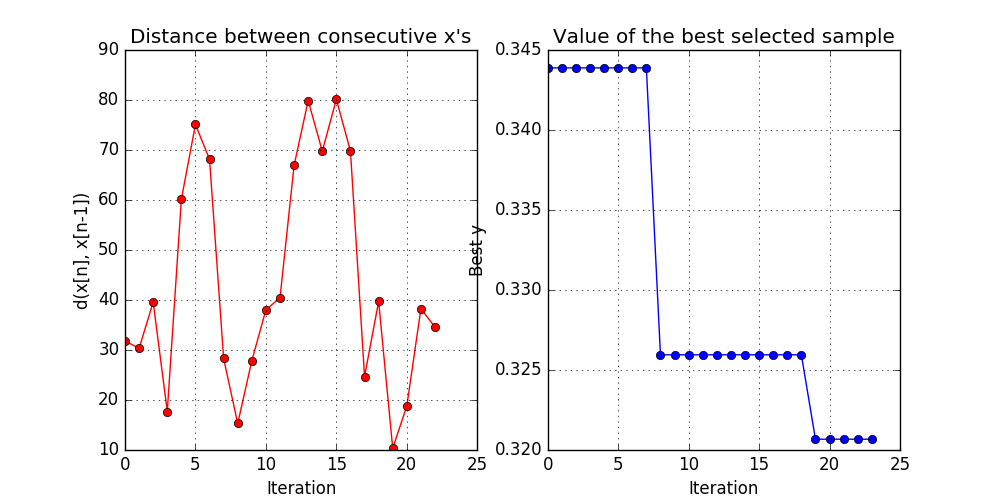
\includegraphics[width=\linewidth]{EIX_CNN_X_init2_STD_ITER60min_v2.png}
	\caption{CNN with EI on 60 minutes budget}
\end{figure}
\begin{figure}[!h]
	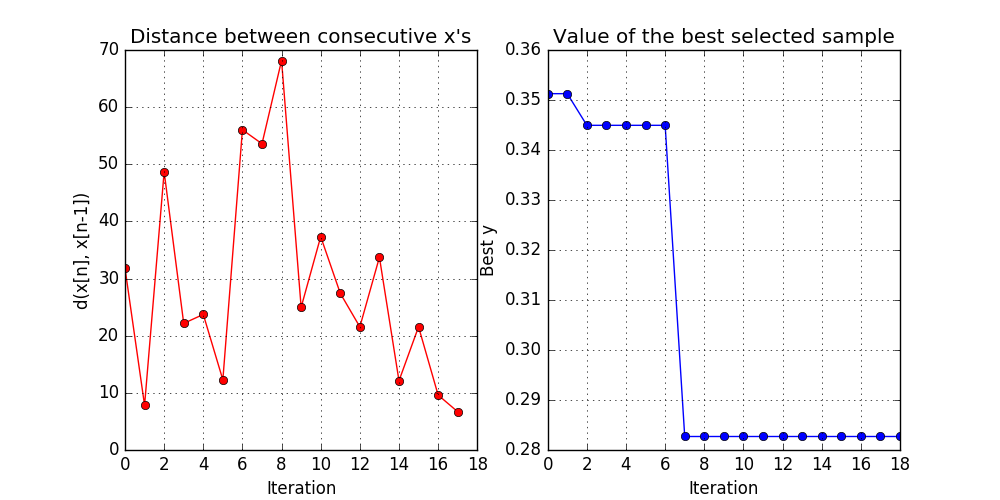
\includegraphics[width=\linewidth]{RAND_CNN_X_init2_STD_ITER60min_v2.png}
	\caption{CNN with Random Search on 60 minutes budget}
\end{figure}
\begin{figure}[!h]
\begin{center}
	\begin{tabular}{lllll}
		\hline
		Cost Model & Acquisition & Best & Best Iter. & Max Iter.\\
		\hline
		\multirow{3}{*}{Std. Cost} & EI &  0.6793 & 19 & 23\\
		& EI-EEC & 0.6663 & 16 & 25\\
		& Random & \textbf{0.7120} & 9 & 18\\
		\hline
		\multirow{4}{*}{No Cost} & EI & \textbf{0.7465} & 37 & 40\\
		& PI & 0.7420 & 29 & 40\\
		& Random & 0.7130 & 22 & 40\\
		\hline
	\end{tabular}
\end{center}
	\caption{CNN validation results}
\end{figure}
The CNN standard cost evaluations were ran with a one hour budget while the no cost evaluations were capped at a maximum of 40 iterations.

While the BO approaches were able to run more iterations, the results were disappointing compared to random search.
We think that this was due to the time model over penalizing expensive hyperparameters.

The performance of the BO approaches are noticably better than random search on 40 iterations.

\vfill\eject
\subsection {Support Vector Machine}
\begin{figure}[h]
	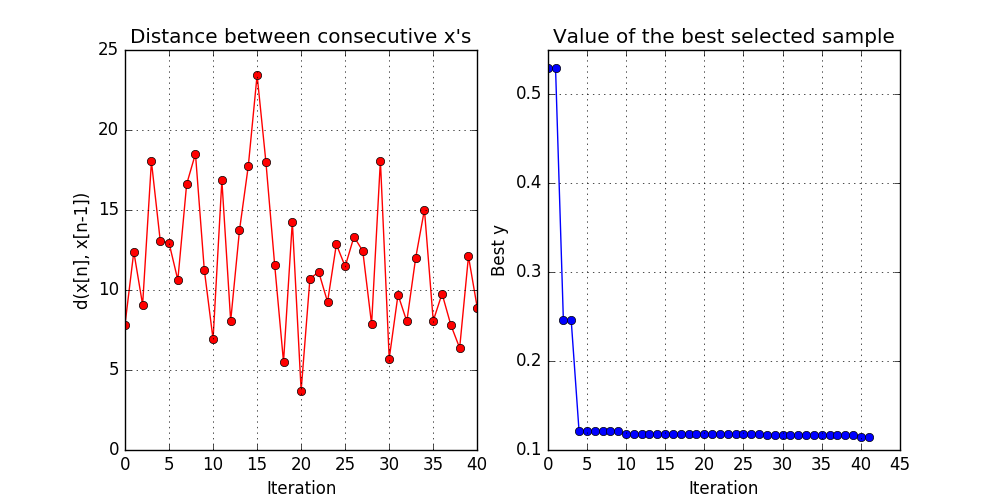
\includegraphics[width=\linewidth]{EIX_SVM_X_init2_NC_ITER40.png}
	\caption{SVM with Probability of Improvement acquisition on 40 iterations}
\end{figure}
\begin{figure}[h]
	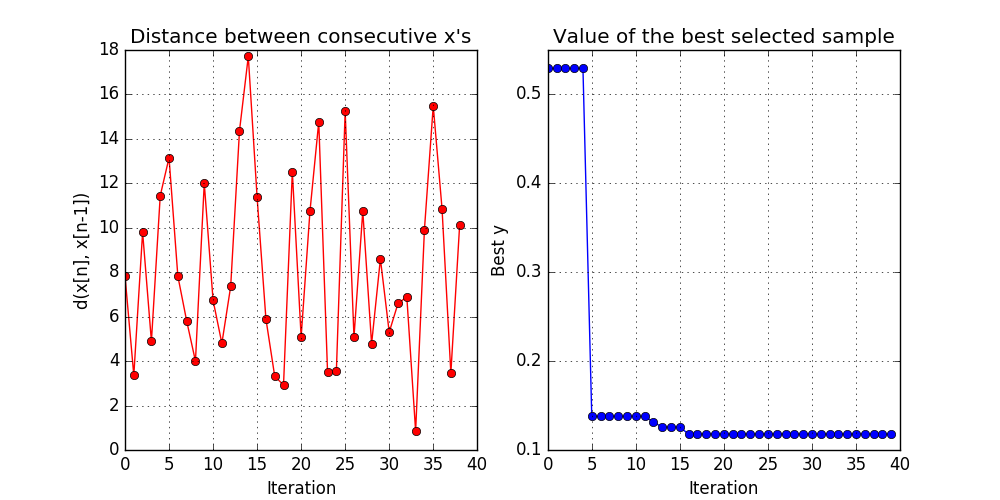
\includegraphics[width=\linewidth]{RAND_SVM_X_init2_NC_ITER40.png}
	\caption{SVM with Random search on 40 iterations}
\end{figure}
\begin{figure}[h]
\begin{center}
	\begin{tabular}{lllll}
		\hline
		Cost Model & Acquisition & Best & Best Iter. & Max Iter.\\
		\hline
		\multirow{3}{*}{Std. Cost} & EI &  \textbf{0.8900} & 51 & 73\\
		& EI-EEC & 0.8850 & 56 & 69\\
		& Random & 0.8864 & 6 & 74\\
		\hline
		\multirow{5}{*}{No Cost} & EI & 0.8842 & 25 & 40\\
		& EI-EEC & 0.8850 & 40 & 40\\
		& PI & 0.8821 & 29 & 40\\
		& MES & \textbf{0.8857} & 28 & 40\\
		& Random & 0.8821 & 16 & 40\\
		\hline
	\end{tabular}
\end{center}
	\caption{SVM validation results}
\end{figure}
The SVM standard cost evaluations were ran with a 10 minutes budget while the no cost evaluations were capped at a maximum of 40 iterations.

An interesting observation is that random search managed to run more iterations than its acquisition-based counterparts.
We believe this is because the time needed to train a SVM does not scale with $\gamma$ or $\textit{C}$.
In addition, a BO iteration requires much more calculations to determine the next set of hyperparameters than a random search iteration.

We also observed that BO and random search have similar performance.
This was likely due to the problem being too simple which makes it easy to hit a good set of hyperparameters by chance.
Still, we can see that BO was able to gain improvements much deeper into the iterations as compared to random search.

\section{Improvements}
\begin{description}
\item [GP hyperparameters and prior] Specification of the Gaussian process prior and better optimisation of its 
hyperparameters are important aspects that we did not have time to investigate.
\item [Using non-stationary kernel] In hyperparameter tuning, the search space is most likely non-uniform and 
non-stationary across the input space. One way is to use non-stationary
kernels or to convert the Matern kernel into a non-stationary kernel.
\cite{shahriari2016taking} Applying a parametric warping
function followed by the Matern kernel could potentially improve results by
accounting for this non-stationarity.
\item [Alternative cost modeling] Expected improvement per second may over penalise expensive evaluations that can nonetheless give good accuracy.
An alternative to account for the cost is to balance the explore-exploit behavior by considering the remaining time budget which is inspired by simulated annealing.
As the remaining time decreases, we can decrease the acquisition's preference for exploration or use a acquisition function that exploits more.
This is applicable for acquisition functions with an explore-exploit parameter such as Expected Improvement with Explore-Exploit cycle.
\end{description}

\section{Roles and Contributions}
\begin{description}
\item [Cheong Xuan Hao Filbert]
\item [Gay Ming Jian Davis]
\item [Karen Ang Mei Yi] Motivating application, Research on acquisition functions
and parallelised Bayesian optimisation, Coding of acquisition functions for experiments and Report writing
\item [Quek Chang Rong Sebastian] Crafting of the Convolutional Neural Network and 
selection of its tunable hyperparameters, and report writing
\item [Vincent Seng Boon Chin] Experimental evaluation design, code and report writing
\item [Xu Ruofan] Research on cost-sensitive modelling and Report writing
\end{description}

\bibliographystyle{aaai}
\bibliography{ref}

\end{document}
